\documentclass[a5paper, 11pt, twoside]{book}  % Based on the ECS Thesis style
% \usepackage{graphicx}
\usepackage{makeidx}
\usepackage{graphicx}
\graphicspath{{../figures/}}  % Location of the graphics files
\usepackage{multirow}
% Making R code work!
\usepackage{listings}
\usepackage{color}
\usepackage{hyperref}
\usepackage{booktabs}

\hypersetup{urlcolor=blue, colorlinks=false, hypertexnames=true}  % Colours hyperlinks in blue, but this can be distracting 
\usepackage{cleveref}
\definecolor{dkgreen}{rgb}{0,0.6,0}
\definecolor{gray}{rgb}{0.5,0.5,0.5}
\definecolor{mauve}{rgb}{0.58,0,0.82}

\lstset{ %
  language=R,                % the language of the code
   basicstyle=\normalsize\ttfamily,           % the size of the fonts that are used for the code
%   numbers=left,                   % where to put the line-numbers
%   numberstyle=\tiny\color{gray},  % the style that is used for the line-numbers
%   stepnumber=2,                   % the step between two line-numbers. If it's 1, each line
                                  % will be numbered
%   numbersep=5pt,                  % how far the line-numbers are from the code
%   backgroundcolor=\color{white},      % choose the background color. You must add \usepackage{color}
%   showspaces=false,               % show spaces adding particular underscores
%   showstringspaces=false,         % underline spaces within strings
%   showtabs=false,                 % show tabs within strings adding particular underscores
   frame=false,                   % adds a frame around the code
   rulecolor=\color{white},        % if not set, the frame-color may be changed on line-breaks within not-black text (e.g. commens (green here))
%   tabsize=2,                      % sets default tabsize to 2 spaces
%   captionpos=b,                   % sets the caption-position to bottom
%   breaklines=true,                % sets automatic line breaking
%   breakatwhitespace=false,        % sets if automatic breaks should only happen at whitespace
%   title=\lstname,                   % show the filename of files included with \lstinputlisting;
                                  % also try caption instead of title
  keywordstyle=\color{blue},          % keyword style
  commentstyle=\color{dkgreen},       % comment style
  stringstyle=\color{mauve},         % string literal style
  escapeinside={\%*}{*)},            % if you want to add a comment within your code
  morekeywords={*,...}               % if you want to add more keywords to the set
} 

% Include any extra LaTeX packages required
\usepackage[round,]{natbib}  % Use the "Natbib" style for the references
\usepackage{verbatim}  % Needed for the "comment" environment to make LaTeX comments
\usepackage{wallpaper}
\usepackage{cases}
\makeindex
% \renewcommand{\includegraphics}[2][]{\fbox{#2}} %omits images
\begin{document}
 
\title{Spatial microsimulation: a practical introduction}
% \author{Robin Lovelace --- R.Lovelace at. Leeds. ac. uk}
\pagestyle{myheadings}
\author{Lovelace, Robin\\
\texttt{r.lovelace@leeds.ac.uk}}
\maketitle

\tableofcontents

\chapter{Preface}
<<<<<<< HEAD
% This booklet was written to accompany a two day course of the same title.
% As well as providing useful information to the $\approx$30 participants during
% and after the course, it is hoped that the material will be of use to others.

\chapter{Introduction}

Spatial microsimulation is shrouded by an unnecessary mystery, and this is not
helped by the fact that most academic papers on subject and even textbooks
lack reproducible examples. In today's age of fast
=======
The trigger for this book's creation was a two day course, An
Introduction to Spatial Microsimulation with R, held at the University
of Leeds in the spring of 2014. Based on the high demand before the course
and feedback from participants taking part, it seemed there was a
definite need for more practical teaching material on spatial microsimulation
than was available at the time: many people had read the literature and had
a good idea about the problem that they wanted to harness the method to solve.
Yet the majority were dissatisfied with the \emph{practical} content of existing
work, or lack thereof.

This book is for all those struggling to find material clearly and succinctly
explaining how to implement spatial microsimulation on their own
datasets.

The underlying motivations for this work go much deeper and are best understood with
reference to my own experience of trying to learn spatial microsimulation. I, like many PhD students
and researchers, was tasked with implementing the method when it was almost completely new to me.
I had barely heard of the method, let alone understood the methodology.
The first stage was to read up on what spatial microsimulation
actually was: in this area I was fortunate enough to have good guidance from my
supervisor Dimitris Ballas, who pointed me towards an accessible introduction to
spatial microsimulation commissioned by the Joseph Roundtree Foundation \citep{Ballas2005b}.
Without this text, I'd have been even more bewildered; overcoming this
bewilderment is a central aim of this course. It will not demonstrate how,
exactly, to apply the method to your own datasets, but it will provide strong
foundations that should enable the method to be applied to almost any combination
of individual and aggregate level datasets, provided suitable shared variables between the two.
As emphasised in the closing chapter of the book, it is the responsibility of
the researcher to ensure that the method is applied in a rigorous and ethical way:
this cannot be taught, although the extensive CakeMap example will demonstrate how
the method can be used in rather absurd ways.

In addition to good guidance towards introductory reading, another major benefit
I had was having Malcolm Campbell as my predecessor. Malcolm provided a huge amount of
support during the early phase of my PhD and shared the entirety of the R code he developed
to perform spatial microsimulation on his Scottish health data.
Not only was the code invaluable to my efforts to build a spatial microsimulation model in
R (some of the code in the book is probably his at some level), his example of collaboration
and code sharing was truly inspirational. Thus this book owes as much to Malcolm as to anyone else
and its free distribution under the Creative Commons license is partly a result of his
generosity in sharing code and enthusiasm of teaching tricky statistical techniques.

% \chapter{Introduction}
\chapter{What is spatial microsimulation?}
Spatial microsimulation is shrouded by an unnecessary mystery, and this is worsened
by much of the literature on the subject. Most academic papers and even some textbooks
about spatial microsimulation lack reproducible examples. In today's age of fast
>>>>>>> 5621fcd28636b3e0bc6e52374ed365f16f97b5ad
Internet connections, open access datasets and free software,
things need not be this way. One could argue that the lack of
reproducibility in spatial microsimulation is damaging to the growth
and credibility of the field.

To those doubting the value of this practical approach, I ask the following
questions: If only a small community of researchers hold the majority of the
code needed to perform spatial microsimulation, how can the technique spread
rapidly to other applications? If every PhD student undertaking spatial
microsimulation must start from scratch, how are the methods going to be
refined and improved in a systematic fashion? Most importantly, if the results
of most spatial microsimulation research is not reproducible --- as is currently
the case --- how can we trust them?

This final point is critical not only to spatial microsimulation but the
disciplines of which it is part. Reproducibility is a prerequisite of
falsifiability --- if the method
underlying a result cannot be replicated by others, how can the finding
possibly be falsified? Moreover, the argument continues, any knowledge or
theory can only claim to enter the realm of `science' if it cannot be falsified.
Because it is impossible to prove any proposition in every and all cases, the
only reliable test we can apply is whether or not it can be \emph{disproved}:
falsified via a contradictory finding. This is how scientific progress is made
\citep{Popper1959}. By writing non-reproducible research, researchers may
inadvertently damage the disciplines in which they work. %. how???

Despite and because of these philosophical antecedents, the course is
unashamedly practical. The aim is simple: to provide an accessible yet
deep foundation in spatial microsimulation. This involves both
\emph{understanding} and \emph{implementation} of the technique.
Following the `learning by doing' ethic, the former can best be
attained through the latter: spatial microsimulation need not be an abstract
process that one simply reads about. It can be practical tool used by anyone
with the know-how. As \citet[xxii]{kabacoff2011r} put it regarding R, ``the best
way to learn is to experiment'' and the same applies to spatial microsimulation.

The examples presented below were developed during a PhD project in the energy
costs of commuting. Although some of the code and most of the descriptive text
has been rewritten since then, many of the ideas and methods are described in
more detail in the resulting thesis.% \citep{Lovelace2014-thesis}.

\chapter{Applications}

\chapter{Spatial microsimulation with R}

\section{Why R?} \label{setsim} % Move this to just before R implementation?

Software decisions have a major impact on the model's flexibility, efficiency,
reproducibility and
ease of coding. \citet[p.~153]{Holm1987} observed that ``little attention is
paid to the choice of programming language used.''
This appears to be as true now as it was then: software is rarely discussed in
spatial microsimulation papers. 
In my own spatial microsimulation research, a conscious decision was made early
on to use R, with impacts on model features, analysis
and even design. It is thus worth understanding the tool a little before we
begin to use it. The theory is discussed in \cref{s:theory}

% \subsection{Why R?}
The world is awash with computer programming languages and many of these
are general purpose and `Turing complete', meaning they could, with sufficient
effort, perform spatial microsimulation. So why would one chose R?
The most important criteria of evaluation include flexibility,
speed of processing and, most importantly, ease and speed of writing code.
R excels in each of these areas, especially the final one: it
is possible to say a lot in R in few lines of code. Further
are provided by \citet{Matloff-R}:

\begin{itemize}
\item ``a public-domain implementation of the widely-regarded S statistical
language; R/S is the de facto standard among professional statisticians
\item comparable, and often superior, in power to commercial products in most
senses
\item available for Windows, Macs, Linux
\item in addition to enabling statistical operations, it's a general programming
language, so that you can
automate your analyses and create new functions
\item object-oriented and functional programming structure
\item your data sets are saved between sessions, so you don't have to reload
each time
\item open-software nature means it’s easy to get help from the user
community''
\end{itemize}
% Add in disadvantages here.

\section{Learning the R language}

<<<<<<< HEAD
Having learned a little about \emph{why} R is a good tool for the job,
it is time to think about \emph{how} R should be used. The most
useful advice I received on the subject is to think of R not as a
series of isolated commands, but as an interconnected \emph{language},
in the fullest sense of the word. R is not only a system by which
instructions can be sent to a computer to process data; R provides a way
of expressing oneself and explaining ideas to other human beings.
Critical to its role as a language is R's unique \emph{syntax}, which allows it
to express relatively complex expressions efficently, with a small number of
keystrokes.
=======
\begin{lstlisting}[float=h, caption={Creating arrays of weights in R},
label=cws]
weights0 <- array(dim=c(nrow(USd),nrow(all.msim)))
weights1 <- array(dim=c(nrow(USd),nrow(all.msim)))
weights2 <- array(dim=c(nrow(USd),nrow(all.msim)))

weights0[,] <- 1 # sets initial weights to 1

USd.agg <- array(dim=c(nrow(all.msim),ncol(all.msim)))
USd.agg1 <- array(dim=c(nrow(all.msim),ncol(all.msim)))
USd.agg2 <- array(dim=c(nrow(all.msim),ncol(all.msim)))
colnames(USd.agg1) <- category.labels
\end{lstlisting}

It is important to note that in real survey data, the variables are not
always neatly categorised into the same bins as the levels of the aggregate
data. Age, for example can be classified in many different ways.
Also, a wide form is useful for subsequent steps.
Therefore, it is necessary to convert the `thin' survey dataset
into a wider form, by converting a single column such as age or sex into
multiple columns corresponding to the number of categories. Sometimes the
cut-off points of the categories can be decided (as with age), or categories
can be merged (when many different NA options are available, for example).
The code that performs this important process for our example dataset is
presented in listing \ref{ccat}.

\begin{lstlisting}[float = h, caption={R code to convert the survey
dataset into binary form}, label=ccat]
USd.cat <- array(rep(0), dim=c(nrow(USd),
			  length(category.labels !=0)))

USd.cat[which(USd$age < 50),1] <- 1 # Age, "< 50"
USd.cat[which(USd$age >= 50),2] <- 1 # "50+"
USd.cat[which(USd$sex =="m"),3] <- 1 # Sex constraint: "m"
USd.cat[which(USd$sex =="f"),4] <- 1 #"f"
sum(USd.cat) # Should be 10
\end{lstlisting}

Another important step shown in \cref{s:theory} was that of converting the
`long' survey dataset into a form that can be compared directly with the
aggregated constraint variables. Listing \ref{cconv} shows how this is done
in R, and the code needed to view the results. (Notice that the first row
of all.msim is the same as those displayed in \cref{t:s})

\begin{lstlisting}[float=h, caption={R code to aggregate the survey dataset},
label=cconv]
 for (i in 1:nrow(all.msim)){ # Loop creating aggregate values 
  USd.agg[i,]   <- colSums(USd.cat * weights0[,i])
}

# Test results
USd.agg

##      [,1] [,2] [,3] [,4]
## [1,]    2    3    3    2
## [2,]    2    3    3    2
## [3,]    2    3    3    2
## [4,]    2    3    3    2
## [5,]    2    3    3    2

all.msim

##   16-49 50+ m f
## 1     8   4 6 6
## 2     2   8 4 6
## 3     7   4 3 8
## 4     5   4 7 2
## 5     7   3 6 4

plot(as.vector(as.matrix(all.msim)),
  as.vector(as.matrix(USd.agg)), xlab = "Constraints",
    ylab = "Model output")
abline(a = 0, b = 1)
\end{lstlisting}

With the data loaded and processed into comparable formats, one is in a
position to start comparing how well our individual level survey dataset
fits with the aggregate constraints (see listing \ref{cconv}). Note that for USd.agg,
the results are the same for every zone, as each individual has a weight of 1
for every zone. Note also the very poor fit between the variables at the
aggregate level, as illustrated by poor correlation between the constraint and
microdata variables (r = 0.05), and a plot of the fit presented in \cref{fct1}.
The next stage is to apply the first constraint,
to adjust the weights of each individual so they match the age constraints
(listing \ref{ccon1} --- note that the top row USd.agg1 is the same as
\cref{t:m2}). After this operation, the fit between the constraint
variables and the aggregated microdata are far better (r = 0.67), but there
is still a large degree of error (\cref{fc1}).

\begin{figure}[h]
 \begin{center}
   
\includegraphics[width = 10cm]{unnamed-chunk-5}
 \end{center}
\caption[Scatter plot of the fit between census and survey data]
{Scatter plot of the fit between census and survey data. This plot
can be re-created using the plot command in listing \ref{cconv}.}
 \label{fct1}
\end{figure}

\begin{lstlisting}[float=h, caption={Reweighting of first constraint
and testing of results}, label=ccon1]
for (j in 1:nrow(all.msim)) {
 weights1[which(USd$age < 50),j] <- all.msim[j,1]/USd.agg[j,1]
 weights1[which(USd$age >= 50),j] <- all.msim[j,2]/USd.agg[j,2]
}
# Aggregate the results for each zone
for (i in 1:nrow(all.msim)) {
 USd.agg1[i,] <- colSums(USd.cat * weights0[,i] * weights1[,i])
}
# Test results
USd.agg1
##      16-49 50+     m     f
## [1,]     8   4 6.667 5.333
## [2,]     2   8 6.333 3.667
## [3,]     7   4 6.167 4.833
## [4,]     5   4 5.167 3.833
## [5,]     7   3 5.500 4.500

plot(as.vector(as.matrix(all.msim)),
 as.vector(as.matrix(USd.agg1)), xlab = "Constraints",
 ylab = "Model output")
abline(a = 0, b = 1)
\end{lstlisting}

\begin{figure}[h]
 \begin{center}
  
\includegraphics[width=10cm]{unnamed-chunk-6}
 \end{center}
\caption{Scatter plot showing the fit after constraining by age.} \label{fc1}
\end{figure}

We will perform the same checks after
each constraint to ensure our model is improving.
To see how the weights change for each individual for each area,
one simply types \verb weights1 , for constraint 1 (listing \ref{cmat}).
Note that the first column of weights 1 is the same as \cref{t:s}.
\begin{lstlisting}[caption = {The new weight matrix. Previously all weights were set to one.},
label =cmat]

##       [,1]  [,2]  [,3]  [,4] [,5]
## [1,] 1.333 2.667 1.333 1.333  1.0
## [2,] 1.333 2.667 1.333 1.333  1.0
## [3,] 4.000 1.000 3.500 2.500  3.5
## [4,] 1.333 2.667 1.333 1.333  1.0
## [5,] 4.000 1.000 3.500 2.500  3.5
\end{lstlisting}

To further improve the fit, one next constrains by the second aggregate constraint:
sex (listing \ref{con2}). To check that our implementation in R produces the
same results as the hand-calculated example, the resulting weights where queried.
As shown by \verb weights3[,1] , these are the same as
those calculated for $w(3)$ above.

\begin{lstlisting}[float=h, caption={Code to constrain the weights by
sex}, label=con2]
for (j in 1:nrow(all.msim)) {
    weights2[which(USd$sex == "m"),j] <-
		  all.msim[j,3]/USd.agg1[j,3]
    weights2[which(USd$sex == "f"),j] <-
		  all.msim[j,4]/USd.agg1[j,4]
}

weights3 <- weights0 * weights1 * weights2
for (i in 1:nrow(all.msim)) {
  USd.agg2[i,] <- colSums(USd.cat * weights3[,i])
}

weights3[,1]

## [1] 1.2 1.2 3.6 1.5 4.5
\end{lstlisting}

The model fit improves greatly after constraining for sex (r = 0.992).
However, to ensure perfect fit more iterations are needed. Iterating
just once more, as done on the online version of this
section\footnote{See
\href{http://rpubs.com/RobinLovelace/6193}{rpubs.com/RobinLovelace/6193}
}
results in a fit that is virtually perfect (\cref{fexits}). More iterations
are needed for larger datasets with more constraints to converge.

\begin{figure} \begin{center}
 
\includegraphics[width = 6cm]{unnamed-chunk-8}
 
\includegraphics[width = 6cm]{unnamed-chunk-11}
 \end{center}
 \caption[Improvement of model fit with iterations]
 {Improvement of model fit after constraining by sex (left)
 and after two complete iterations (right).} \label{fexits}
\end{figure}

The worked code example in this section is replicable.
If all the code snippets are entered, in order, the results
should be the same on any computer running R. There
is great scope for taking the analysis further:
some further tests and plots are presented on the on-line
versions of this section. The simplest case is contained in
Rpubs document \href{http://rpubs.com/RobinLovelace/6193}{6193} and a more
complex case (with three constraints) can be found in Rpubs document
\href{http://rpubs.com/RobinLovelace/5089}{5089}. The preliminary checks
done on this code are important to ensure the model is understood
at all times and is working correctly. More systematic methods
for model checking are the topic of the following section.

\chapter{Customising code: a worked example with CakeMap data}


\chapter{The Flexible Modelling Framework (FMF)}

\section{Model checking and validation} \label{smeval}

To make an analogy with food safety standards, openness about mistakes is
conducive to high standards \citep{Powell2011}. Transparency in model
verification is desirable for similar reasons. The two main strategies are 1) 
comparing the model results with knowledge of how it \emph{should}
perform \emph{a-priori} (model checking) and 2) comparison between the model
results and empirical data (validation).

\subsection{Model checking}
A proven method of checking that data analysis and processing is working
is wide ranging and continual visual exploration of its output
\citep{janert2010data}.
This strategy has been employed
throughout the modelling process, both to gain a better understanding of the
behaviour of the underlying R code, and to search for unexpected
results. These were often precursors to error identification.

An example of this, that illustrates the utility of ad-hock checks, is the
continual plotting of model inputs and outputs to ensure that they
make sense. The R commands \verb summary() \ and \verb plot() \ are ideal for
this purpose. The former provides basic descriptive statistics; the latter
produces a graphical display of the object. Both are \emph{polymorphic},
meaning that command adapts depending on the type of object it has been asked
to process \citep{Matloff-R}. Thus, to check that
the number of people in each age and sex category in the input and output
dataset made sense overall, the
following command was issued, resulting in the plot illustrated in \cref{fasp}:

\begin{lstlisting}
plot(cut(USd$age, breaks=(seq(0,100,20))), USd$sex)\end{lstlisting}
% TAKEN FROM ~/Dropbox/vul-meth/etsimY

\begin{figure}[h]
 \begin{center}
   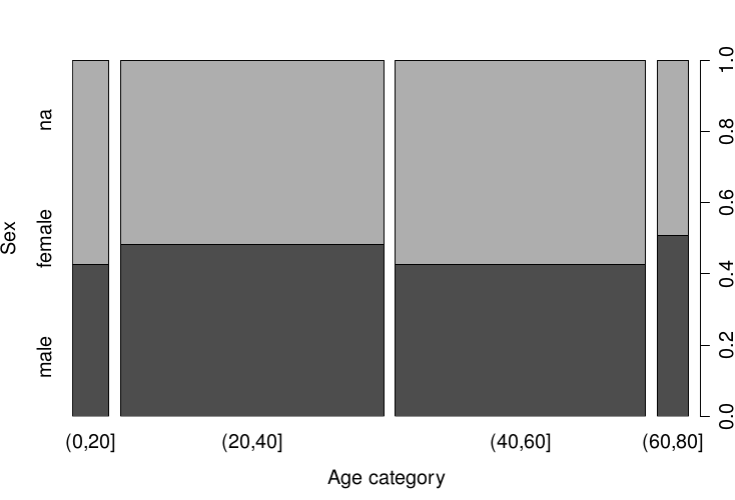
\includegraphics[width = 12cm]{age-sex-plot}
 \end{center}
 % cc-ems.pdf: 792x612 pixel, 72dpi, 27.94x21.59 cm, bb=0 0 792 612
\caption[Diagnostic plot to check the sanity of age and sex inputs.]{Diagnostic
plot to check the sanity of age and sex inputs. (Square brackets
indicate that the endpoint is not included in the set --- see
International Organization for Standardization
\href{http://www.iso.org/iso/catalogue_detail?csnumber=31887}{(ISO) 80000-2:2009},
formerly \href{http://en.wikipedia.org/wiki/Interval_(mathematics)}{ISO 31-11}
on ``mathematical signs and symbols for use in physical sciences and technology'').}
 \label{fasp}
\end{figure}
These common-sense methods of data checking may seem overly simplistic to warrant
mention. Yet such basic sanity tests are the `bread-and-butter' of
quantitative analysis. They ensure that the data are properly
understood \citep{Wickham2008}. Had the input data represented in \cref{fasp}
contained an equal proportion of people under 20 as over 20, for example,
one would know that the input data for commuters was faulty.
This approach, whereby major
problems are revealed early on in frequent tests, is preferable to waiting
until the results of the full spatial microsimulation are analysed. Hours were
saved, and understanding of the input datasets was improved.\footnote{The
use of the
same command to check model output was crucial to the identification of
important errors, including a small mistake in the code which led to large
errors in the synthetic microdata output for the distance constraint variables.}

The basic tenet of spatial microsimulation is that simulated and actual data
should match at the aggregate level \citep{Ballas2007simb}.
This knowledge led to the
continual plotting of census vs simulated results in the early stages of the
model construction, and the development of more
sophisticated plots (see \cref{fig:IPF-4c}).
Still, the humble scatter plot was used frequently for
preliminary analysis. To provide an example, after the model was run for
Yorkshire
and the Humber region for 20 iterations, I was confident the results were
correct: the results had been tested for Sheffield, and everything
\emph{seemed} to be working as expected.

Knowledge of how model-census fit should look started alarm bells
ringing when an imperfect plot was discovered:
% (largely by luck, as I was looking at the fit
% between only some of the variables, and happened to think the number of people
% taking very short trips could be subject to higher than normal levels of
% error). % What does this contribute? Nowt.
\cref{fig:error} (A) was cause for concern, not only for the low
correlation between the two variables (which was still greater than 0.8), but
because the direction of the error: the model had \emph{always} overestimated the
number of people travelling short distances to work in past runs.
This seemed suspicious, and the relationship was plotted for earlier constraints
to identify where the problem was variables were plotted.
\cref{fig:error} (B) was the
result of this, after constraining by distance.
Something had clearly gone wrong because no people who work
from home had been registered in the aggregate output. These issues led to
a re-examination of the code contained
within the file cats.r. It was found that a faulty placement of an
equals sign (such that values ``greater than or equal'' to 0 were accepted as 0
- 2 km travel to work). The problem was solved, and the model correlation
improved as a result (\cref{fig:error} (C)).

The two examples described above provided insight into how the model was
performing by its own standards. The more challenging stage is to validate
the model against factors external to it. % This is further discussed !!!

\begin{figure}[h]
  \begin{center}
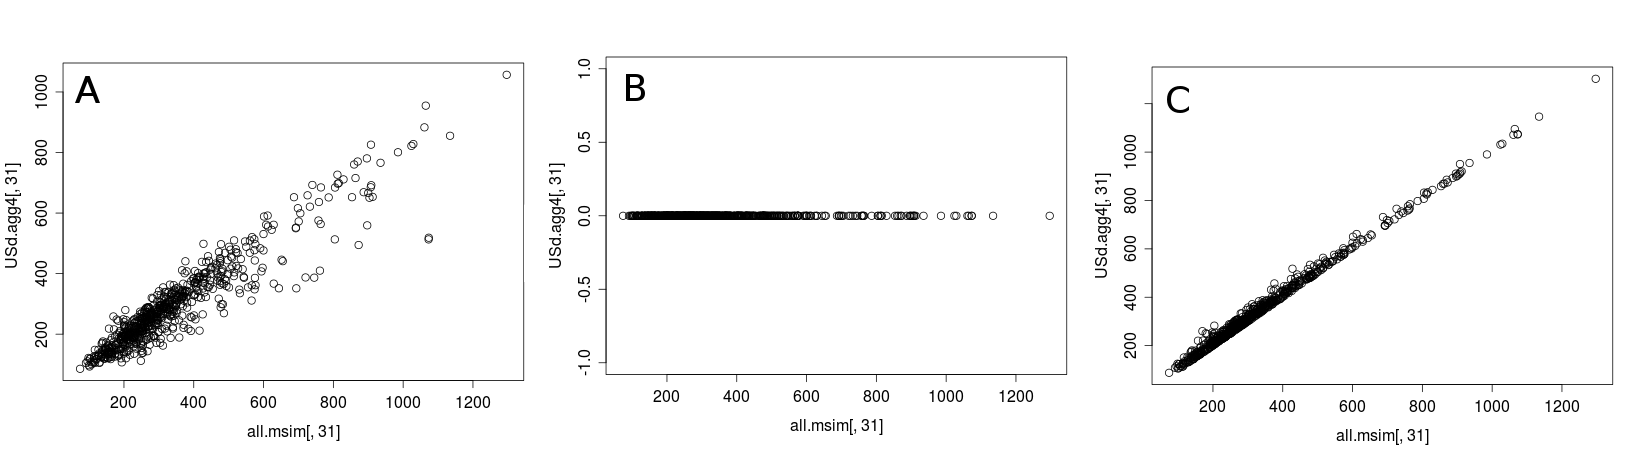
\includegraphics[width=15cm]{errors3-1}      \end{center}
 % cc-trans.png: 1113x529 pixel, 72dpi, 39.26x18.66 cm, bb=0 0 1113 529
 \caption[Diagnostic plots to identify model error]{Three diagnostic plots used
to identify a code error in the spatial microsimulation model (for the
distance category `travels 0--2 km to work'). The x-axis is
census data, the y-axis is the simulated result. A) First plot
analysed (for iteration 20); B) second plot, which illustrated the source of the
problem, in the distance constraint; C) satisfactory diagnostic plot,
after the problem had been resolved.}
 \label{fig:error}
\end{figure}

\subsection{Model validation}
\label{meval}
% {\color{red} Should this section be in a later chapter?} !!!
Beyond `typos' or simple conceptual errors in model code, more fundamental
questions should be asked of spatial microsimulation models. The validity
of the assumptions on which they are built, and the confidence one should have
in the results are important. This is especially true of models designed to inform
policies which have the potential to influence quality of life. Yet
evaluation and `validation' are
 problematic for any models that attempt to explain extensive, complex
systems such as cities or ecosystems. The urban modelling approach, of which
spatial microsimulation of commuters is a subset, has been grappling with this
problem since its infancy. Lacking a crystal ball, time-machine or settlements
on which controlled experiments can be performed, the difficulty of model evaluation can
seem intractable: ``only through time can a model be verified in any
conventional sense of the word'', by comparing the range of projected futures
with the reality of future change in hindsight \citep[p.~15]{batty1976urban}.

Why do urban models pose such a problem? Previously unknown knock-on impacts
cannot be ruled out due to the vast number of links between system
elements.\footnote{It is, of course, impossible to know how every resident of
an area interacts with every other, let alone predict the future impacts of
this interaction, even in the era of ubiquitous digital communications.
}
Rigorous real-world testing is usually impossible due to the scale of the system
and ethics involved with intervening in peoples' lives for the sake of research.
Controlled experiments cannot be performed on real settlements in the
same way that experiments can be performed in the physical sciences and, even if
two similar settlements could be found on which to apply different
interventions, there is no guarantee that all other factors will be held
constant throughout the duration of the experiment. %%% Refs!!!
% Going off on a bit of a waffle to be fair

Additional evaluation problems apply to spatial microsimulation models in
particular for a number of reasons, including:
\begin{itemize}
 \item The aggregate values of categorical `small area' constraint variables are already known from the Census, 
 so should be accurate. Checking the distribution of continuous variables such as 
 age and distance travelled to work against these crude categories is 
 problematic.\footnote{For example, if 50\% of
commuters in a particular area travel 2--5 km to work according to the Census,
does that mean that there is a normal distribution of trip distances with the
mean focussed on 3.5? Or is it more likely that there is a single large
employer located somewhere between 2 and 5 km from the bulk of houses in the
area, which accounts for the majority of these jobs and leads to a skewed
distribution of home-work distances. In every event, spatial microsimulation
will ignore such subtleties and smooth out extreme skewness by approximating the
national distance trends within each distance bin.
}
  \item Target variables are not generally known as geographic
aggregates. Therefore checking their validity for small areas is 
difficult: new surveys may be needed.
  \item Spatial microsimulation results in long lists of individuals for each
zone. With thousands of individuals in each zone and hundreds of zones, the
datasets can become large and unwieldy.
\end{itemize}
>>>>>>> 5621fcd28636b3e0bc6e52374ed365f16f97b5ad

The concise and unusual nature of R code
is not an accident. It was planned to be this way from the
outset by its instigators, Robert Gentleman and Ross Ihaka, who thought
carefully about syntax from the outset:
``the syntax of a language is important
because it determines
the way that users of the language express themselves'' \citep[p.~300]{Ihaka2014}.

\section{Typographic conventions}

\section{An overview of the book}


\chapter{What is spatial microsimulation?}

\section{What spatial microsimulation is not}

\section{A method for generating spatial microdata}

\section{An approach to modelling ecological processes}

\section{A tool for combining insights from multiple scales}

\chapter{Applications}


\section{Updating cross-tabulated census data}

\section{Economic forecasting}

\section{Small area estimation}

\section{Transport modelling}

\section{Dynamic spatial microsimulation}

\section{An input into agent based models}

\chapter{Spatial microsimulation in theory}\label{s:theory}


\section{Iterative Proportional Fitting}

<<<<<<< HEAD
\section{Combinatorial optimisation}
=======
Other than the sanity check of age-sex ratios presented in \cref{fasp},
the evaluation methods considered above operate at the level of geographically
aggregated counts. However, the unique feature of spatial microsimulation is
its simulation of individuals. Evaluation techniques should therefore operate
at the individual level as well.
% The potential for evaluation of the simulated
% spatial microdata outputs is limited by the availability of official spatial
% microdata. As a result this section is short and, for the most part,
% purely theoretical.
%
% The available datasets were introduced with reference to an idealised
% `perfect' dataset on commuting \cref{fdata-ideal}. In the same way, we will
% describe methods of evaluating the microsimulation model at the individual
% level with reference to the ideal of unlimited data. This will inform the
% discussion of how best to use the individual level data that is available
% for model evaluation...
Because simulation, almost by definition, estimates something that is not
otherwise known, it is hard to find reliable individual level
data against which the estimates can be evaluated. For this reason
individual level surveys could be conducted in a specific area where
spatial microdata have been generated. To take one example, a randomised
sample of households could be taken in a single ward. Respondents would be
asked the mode of travel to work, distance and frequency of trip and
other variables. This would allow the model to be evaluated
not only in terms of the correlations that it outputs between different categories,
but also for the evaluation of the assumptions on which the energy calculations %??? where
are based.

One of the main advantages %cited where???
of spatial microsimulation over just using aggregated data is that it provides
insight into the \emph{distribution} of continuous variables within each zone,
rather than just counts of categories which are often rather coarse. T-tests and
Analysis of Variance (ANOVA) tests could then be used to check if the
mean and variance of the simulated and survey data are statistically likely
to be from the same population. However, the raw results of IPF are not
conducive to such tests at the individual level because they do not contain
whole individuals. Integerisation of the weight matrices is needed.

\section{Integerisation} \index{integerisation}
A question raised by this research is this: How do integerised IPF results
compare with other (e.g. combinatorial optimisation) approaches to spatial
microsimulation?
Studies have compared non-integer results of IPF with
alternative approaches \citep{harland2012}, but not like-with-like.

\section{Extensions to the basic model}
\label{discuss}

\chapter{Spatial microdata inputs into agent based models}

\chapter{Conclusions and further resources}

\section{Acknowledgements}
>>>>>>> 5621fcd28636b3e0bc6e52374ed365f16f97b5ad

\section{Multilevell modelling}

\chapter{Spatial microsimulation with R}


\section{Loading and cleaning input data}

\section{Comparing individual and aggregate data}

\section{Reweighting using IPF}

\section{Combinatorial optimisation}

\section{Integerisation}

\chapter{Customising code: a worked example with CakeMap}


\section{Preparing the input data}

\section{Performing IPF on CakeMap data}

\section{Integerisation}

\section{Validation}

\section{Visualisations}

\section{Analysis and interpretation}


\chapter{Additional tools and techniques}


\section{The Flexible Modelling Framework (FMF)}

\section{Allocation of home-work locations}

\section{A spatial interaction model with individual agents}

\section{Spatial microdata: an input into agent based models}


\chapter{Conclusions and a peak into the future}

% \section{Acknowledgements}
\chapter{Bibliography}
\label{Bibliography}

\bibliographystyle{plainnat}  
\bibliography{/nfs/foe-fs-01_users/georl/Documents/Microsimulation}  % The
% /nfs/foe-fs-01_users/georl/Documents/Microsimulation,
% /home/robin/Documents/Microsimulation.bib
\addtocontents{toc}{\vspace{2em}}  % Add a gap in the Contents, for aesthetics

%% -----------------------------------------------------------

\printindex
\label{index}
\phantomsection
\addcontentsline{toc}{chapter}{Index}
\end{document}  % The End
